%
% einleitung.tex -- Beispiel-File für die Einleitung
%
% (c) 2020 Prof Dr Andreas Müller, Hochschule Rapperswil
%
% !TEX root = ../../buch.tex
% !TEX encoding = UTF-8
%
\section{Einführung\label{geradlinig:section:einfuehrung}}
\kopfrechts{Einführung}
Im Zeitalter der Industrialisierung stellte sich heraus, 
dass Rotationen mechanisch einfacher zu realisieren sind als Translationen.
Ein Grund war, dass damals geradlinige Bewegung nicht sehr 
natürlich vorkam aufgrund von äusseren Einwirkungen wie z.B. 
Schwerkraft, Reibung etc.
Dadurch etablierte sich die Kreisbewegungen in fast alle Mechanismen
und Antriebsarten.
Aber geradlinige Bewegung wurde immer gefragter, was Ingenieure und
Erfinder im 18 und 19.\,Jahrhundert antrieb sich der Herausforderung
der geradlinigen Bewegung zu stellen.

\subsection{Newcomens Dampfmaschine\label{geradlinig:subsection:newcomen}}
Die erste Maschine die Kraft durch geradlinige Bewegung übertrug 
war Newcomens Dampfmaschine~\cite{wiki_newcomen}, 
gebaut durch Thomas Newcomen im Jahre $1712$.
Sie wurde durch Dampf betrieben, der in den Zylinder gesaugt,
wodurch ein Teilvakuum entstand, das es ermöglichte, dass der Kolben
durch den atmosphärischen Druck in den Zylinder gedrückt wurde.
Damit konnte auf der anderen Seite der Trägerstange Arbeit verrichtet werden.
Somit handelt es sich hierbei auch um die erste Dampfmaschine
illustriert in der Abbildung~\ref{fig:newcomen_engine}.
\begin{figure}[htbp]
    \centering
    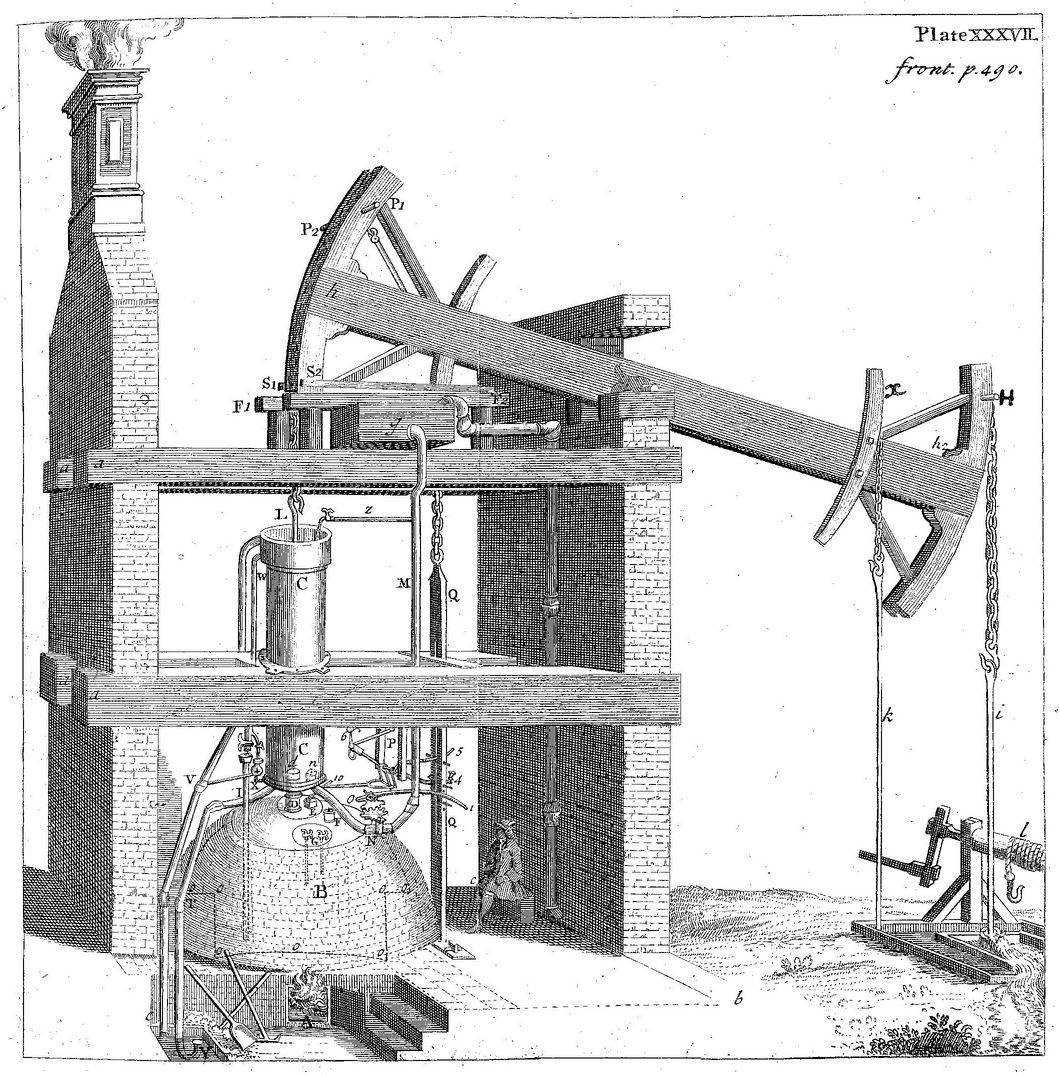
\includegraphics[width=\textwidth]{papers/geradlinig/figures/newcomen_engine.jpg}
    \caption{Illustration von Newcomens Dampfmaschine~\cite{newcomen_pic}.} 
~\label{fig:newcomen_engine}
\end{figure}

\subsection{Watts Dampfmaschine\label{geradlinig:subsection:watts_steam}}
James Watt sah Potential die Newcomen Maschine zu verbessern.
Insbesondere fand er das Prinzip den gleichen Kolben für die Erhitzung und 
Abkühlung zu nutzen sehr ineffizient~\cite{wiki_watt_steam}.
Dafür baute er einen separaten Zylinder für die Kondensation ein.
Nachdem der Arbeitszylinder mit Dampf gefüllt war, 
wurde ein Ventil zum Sekundärzylinder geöffnet, sodass der Dampf in diesen strömen
und dort kondensieren konnte.
Das Ergebnis war derselbe Zyklus wie bei Newcomens Konstruktion, jedoch ohne
jegliche Kühlung des Arbeitszylinders, der somit sofort 
für einen weiteren Hub bereit war.
Danach verbesserte er die Maschine, sodass sie den Zylinder beidseitig mit 
Dampf antrieb, mit ziehen und drücken
Das ging nicht mehr mit einer Kette, deswegen wurde diese mit einer Stange ersetzt.
Zudem war es nicht möglich, die Kolbenstange des abgedichteten Zylinders 
direkt mit dem Träger zu verbinden, 
da sich die Stange zwar vertikal in einer geraden Linie bewegte, 
der Träger jedoch in seiner Mitte schwenkbar gelagert war, 
sodass jede Seite einen Bogen beschrieb.
Diese Vorrichtung, gemäss Abbildung~\ref{fig:watts_engine},
nutzte ein Viergelenkgestänge in Verbindung mit einem Pantographen, 
um die erforderliche geradlinige Bewegung wesentlich kostengünstiger zu erzeugen,
als es mit einem Gleitgestänge möglich gewesen wäre.
Damit hat er die Leistung verdoppelte und sorgte für eine geschmeidigere Übertragung.
Dadurch eignete sich die Maschine ideal, um Räder anzutreiben.
\begin{figure}[htbp]
    \centering
    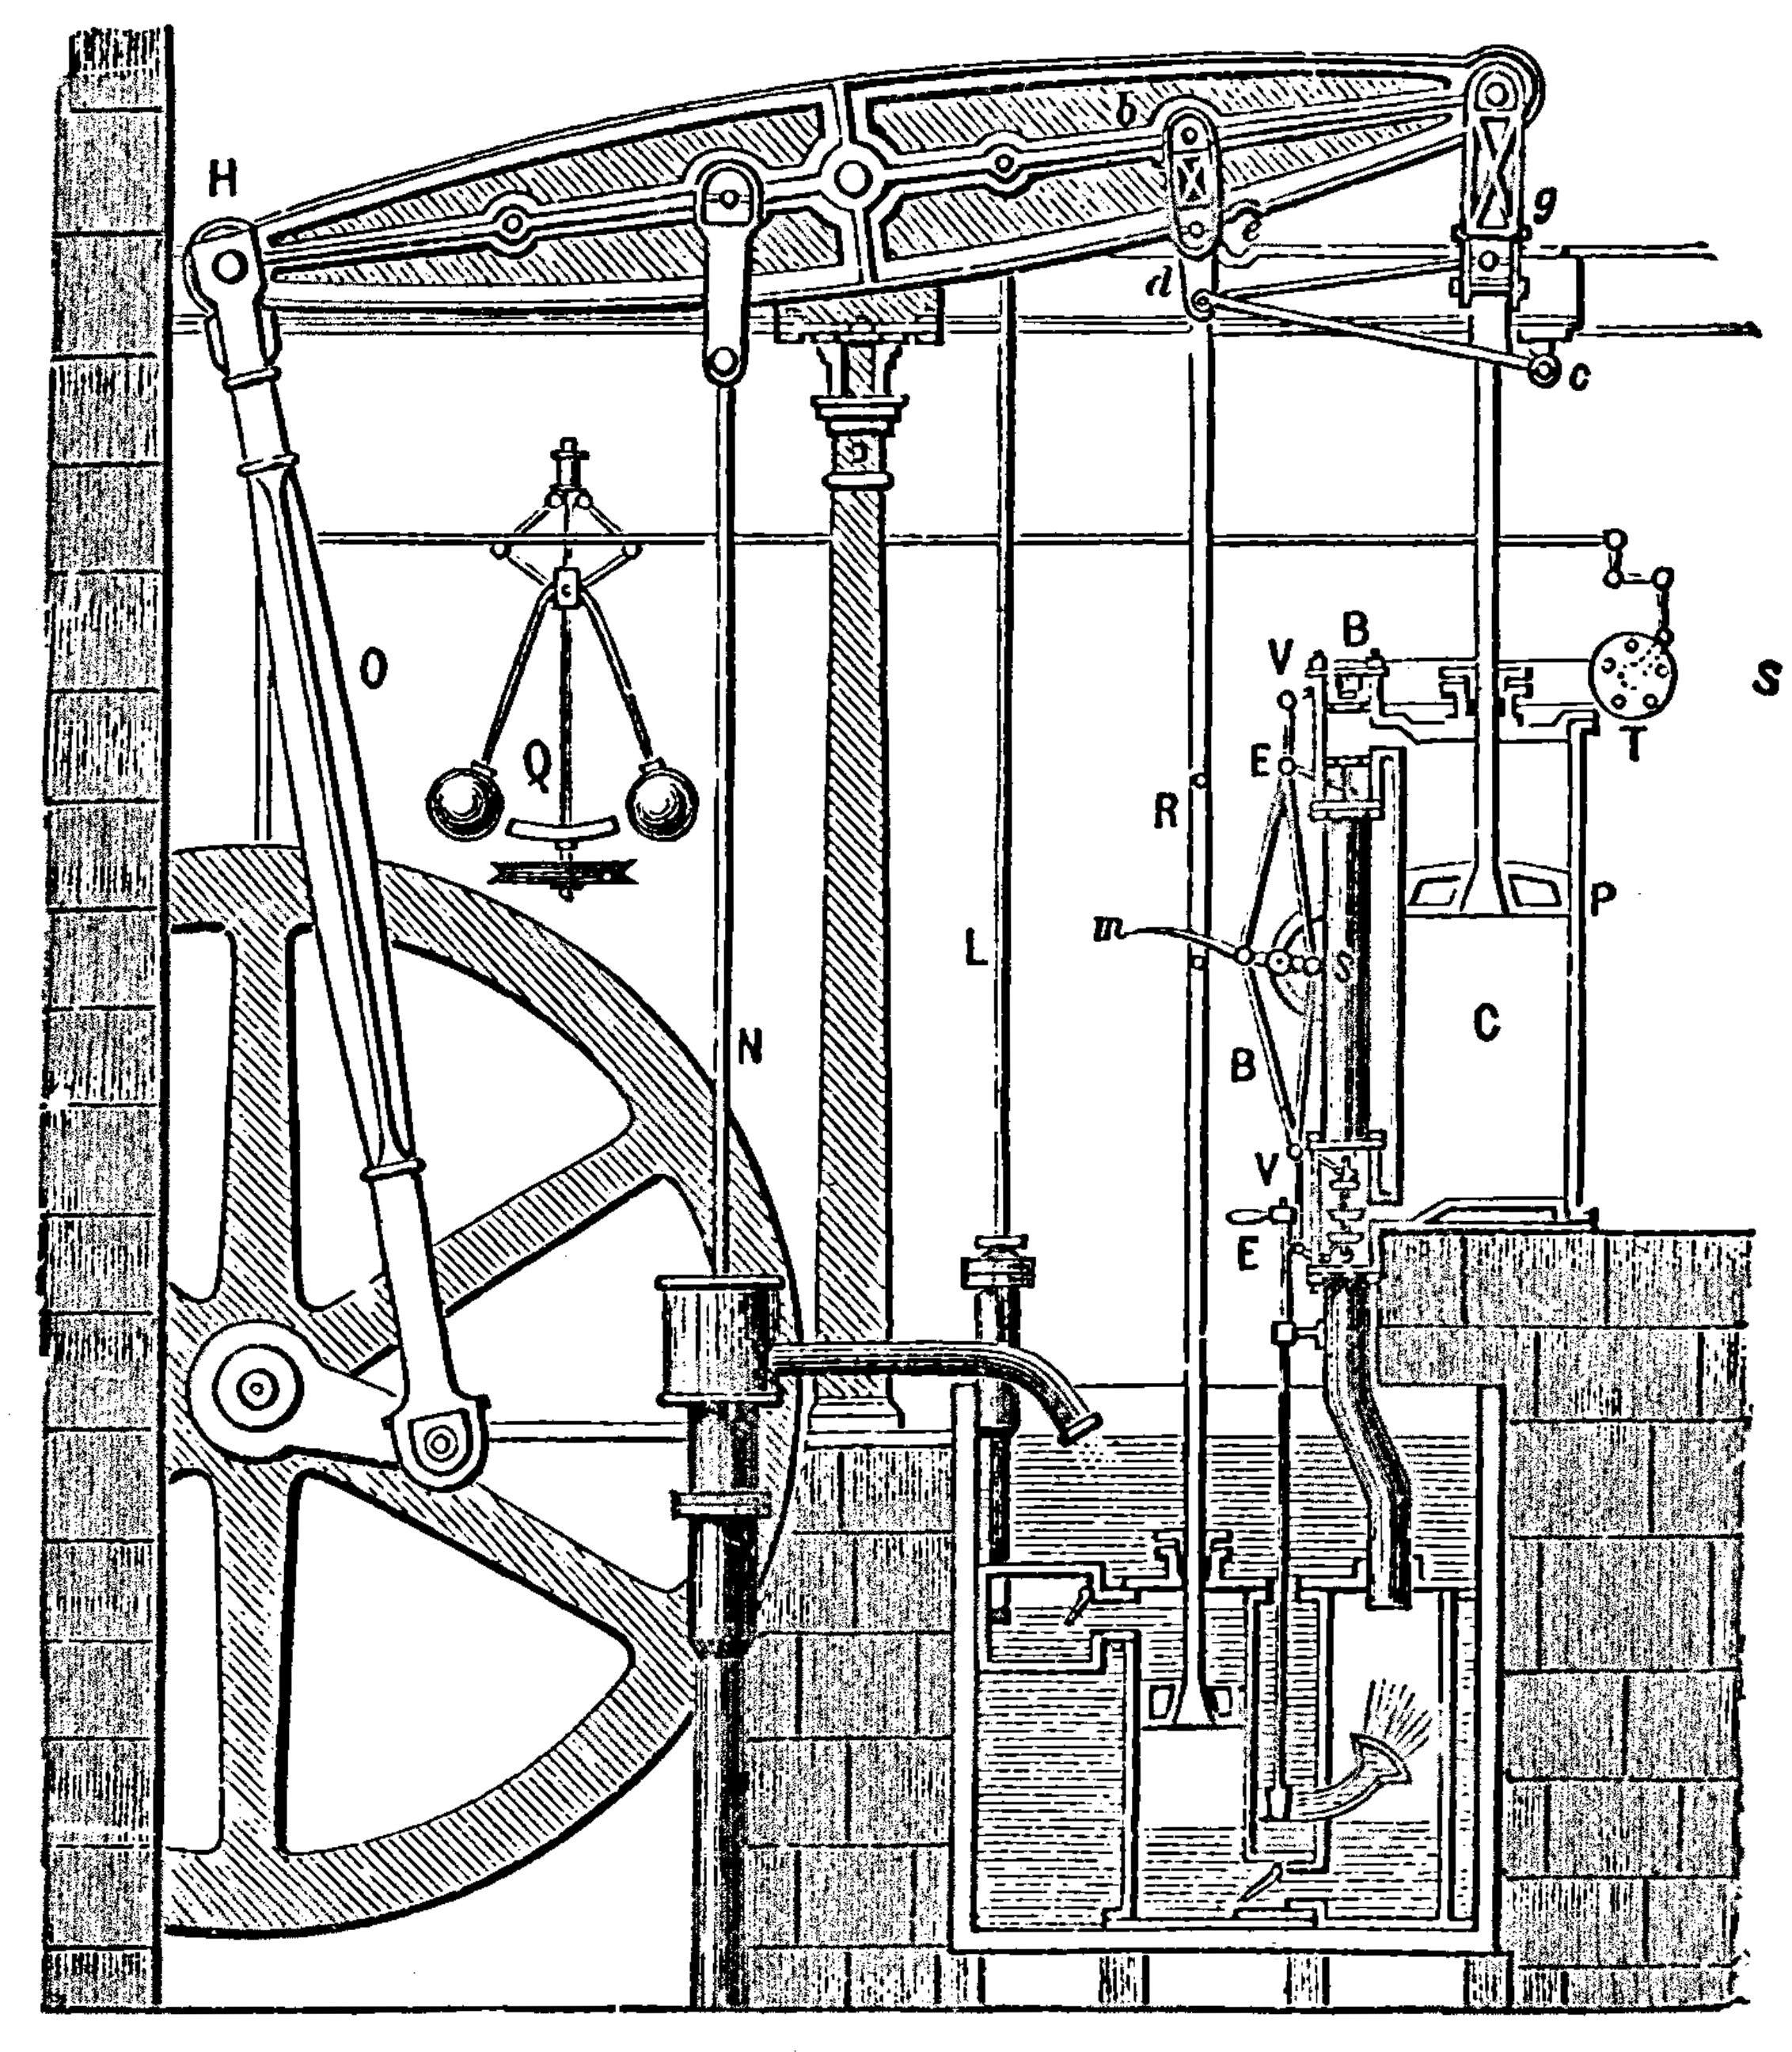
\includegraphics[width=\textwidth]{papers/geradlinig/figures/watts_engine.jpeg}
    \caption{Illustration von Watts Dampfmaschine~\cite{wiki_watt_steam}.} 
~\label{fig:watts_engine}
\end{figure}

\subsection{Kinematische Synthese
\label{geradlinig:subsection:kinematische_synthese}}
Mit seinem Design führte James Watt die kinematische 
Synthese~\cite{kin_synth} ein.
Dabei handelt es sich um das Verfahren zur Bestimmung der Grösse und
Konfiguration von Gelenken um eine gewünschte Bewegung zur erzielen
mit dem Mechanismus.
Einige davon waren nur mathematischer Natur und andere wurden in 
Maschinen und Fahrzeugen umgesetzt.
Die erste Evolution davon waren die Viergelenkgestänge.
In diesem Paper beschränken wir uns ausschliesslich auf die Mechanismen,
welche approximative und perfekte geradlinige Bewegung erzeugen.